\documentclass[10pt]{ctexart}
\usepackage{ylsart}
\usepackage{enumerate}
\usepackage{bm}
\usepackage{makecell}
\usepackage{xcolor}
\usepackage{graphicx}
\usepackage{subfigure}
\usepackage{framed}%包中有添加文字背景色命令shaded
\colorlet{shadecolor}{MaterialBlue50}
\usepackage{tabularx}
\usepackage{multicol}  
\usepackage{multirow}
\usepackage{indentfirst}
\usepackage{amsmath,amssymb,amsthm,bm,bbding,pifont,dsfont}
\usepackage{mathtools}
\newcommand{\abs}[1]{\left| #1 \right|}
\usepackage{caption}
\captionsetup[figure]{labelfont={bf},labelformat={default},labelsep=period,name={图}}
%定义选择题选项
\newcommand{\onech}[4]{
\renewcommand\arraystretch{1.4}
\begin{tabularx}{\linewidth}{XXXX}
\setlength\tabcolsep{0pt}
(A) #1 & (B) #2 & (C) #3 & (D) #4 \\
\end{tabularx}
\unskip \unskip}
\newcommand{\twoch}[4]{
\renewcommand\arraystretch{1.4}
\begin{tabularx}{\linewidth}{XX}
\setlength\tabcolsep{0pt}
(A) #1 & (B) #2 \\
(C) #3 & (D) #4
\end{tabularx}
\unskip \unskip}

\title{模型研究系列 \quad 将军饮马}
\author{安徽省霍邱县第一中学城南分校\\一粒沙}
\date{\today}



\begin{document}
\maketitle
\tableofcontents


\section{引入}

{引入}
“白日登山望烽火,黄昏饮马傍交河”,这是唐代诗人李颀《古从军行》里的一句诗。由此却引申出一系列非常有趣的数学问题,通常称为“将军饮马”.

\section{什么是将军饮马?}
【问题描述】

如图,将军在图中点$A$处,现在他要带马去河边喝水,之后返回军营$B$,问:将军怎么走能使得路程最短?
\begin{center}
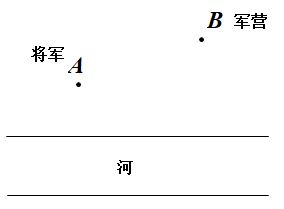
\includegraphics[scale=0.6]{figure/1-1.PNG} 
\end{center}

【问题简化】

如图,在直线上找一点$P$使得$PA+PB$最小?

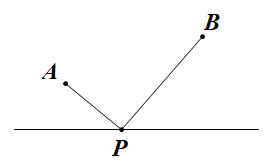
\includegraphics[scale=0.6]{figure/1-2.PNG} 

【问题分析】

这个问题的难点在于$PA+PB$是一段折线段,通过观察图形很难得出结果,关于最小值,我们知道“两点之间,线段最短”、“点到直线的连线中,垂线段最短”等,所以此处,需转化问题,将折线变为直线段.

【问题解决】

作点$A$关于直线的对称点$A'$,连接$PA'$,则$PA'=PA$,所以$PA+PB=PA'+PB$.

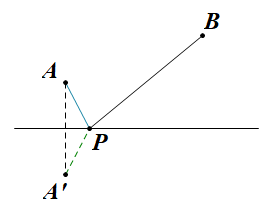
\includegraphics[scale=0.6]{figure/1-3.PNG} 

当$A',P,B$三点共线的时候,$PA'+PB=A'B$,此时为最小值(两点之间线段最短)

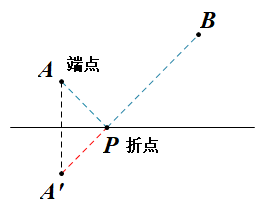
\includegraphics[scale=0.6]{figure/1-4.PNG} 

\section{将军饮马模型系列}
\subsection{“一定两动”之点到点}
在$OA,OB$上分别取点$M,N$,使得$\Delta PMN$周长最小.

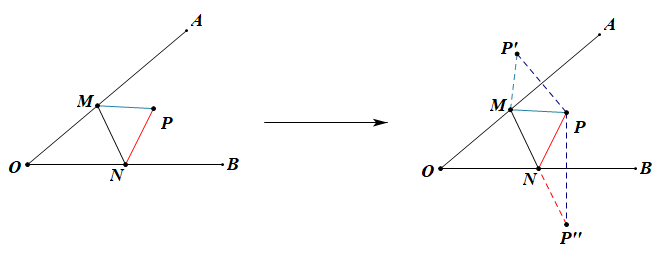
\includegraphics[scale=0.6]{figure/2-1.PNG}
 
此处$M,N$均为折点,分别作点$P$关于$OA$(折点$M$所在直线)、$OB$(折点$N$所在直线)的对称点,化折线段$PM+MN+NP$为$P'M+MN+NP''$,当$P',M,N,P''$共线时,$\Delta PMN$周长最小.

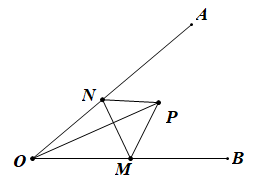
\includegraphics[scale=0.6]{figure/2-2.PNG}
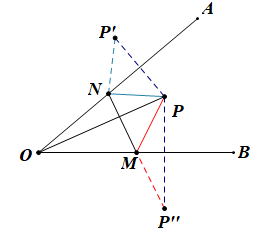
\includegraphics[scale=0.6]{figure/2-3.PNG}
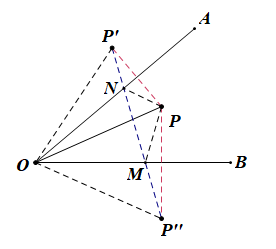
\includegraphics[scale=0.6]{figure/2-4.PNG}
\subsection{“两定两动”之点到点}


\subsection{“一定两动”之点到线}
\section{几何图形中的将军饮马}
\subsection{正方形中的将军饮马}
\subsection{三角形中的将军饮马}
\subsection{菱形、矩形中的将军饮马}

\section{特殊角的对称}
\section{将军过桥}
\section{将军遛马}















\end{document}